\chapter{analysis}\label{analysis}

ToDo:
\begin{enumerate}[nosep]
    \item Datenformat Input, verwendete Daten, Worte zu Simulation, trainingsdaten
    \item Preprocessing - Schritte erklären
    \item Datenformat Output Preprocessing
    \item Signifikanzkurve
\end{enumerate}

\section{Simulated Data and Preprocessing}
% configuration in appendix! + algorithmen beim prep

\subsection{Monte Carlo Data (More Infos: number of events, \ldots)}
Our analysis is based entirely on simulated monte carlo (MC) data.
The particle shower simulation is done with the software CORSIKA, 
the simulation of the instrument response goes by the name of simtel.

Monte carlo data is simulated and shared across the CTA-collaboration, 
our analysis uses the data from the PROD3-simulation of 
the CTA-south array. These simulation include way more telescopes 
than the array will eventually have. This is done to compare
different layouts and telescope positions.
We will choose the relevant telescopes in a way, that
our array resembles the earlier mentioned south array (See section \ref{sec:cta}).

This data contains everything the telescopes are going to measure
at a low level
plus additional MC information, that will not be present at real experiments.
This includes the simulated particle direction and energy and type.
This ground-truth or MC-truth allows us to gauge the efffectiveness of our 
algorithms by comparing the predictions with the MC-truth values.

The total number of simulated data after the low level analysis 
is shown in table \ref{tab:mc_info}. (SIMTEL INFOS? ODER DAS HIER SPÄTER?)

\begin{center}
    \begin{tabular}{| l | l | l | l |}
    \hline
     & Pointlike Gamma & Diffuse Gamma & Protons \\
    \hline
    MC runs & \num{1113} & \num{17382} &  \num{9273} \\ 
    \hline
    Array events & \num{955317} & \num{3409290} & \num{4657529} \\
    \hline
    Telescope events & \num{4554313} & \num{14383270} \num{20106385} & 
    \end{tabular}
    \caption{Take the infos from the simtel files instead! List file sizes aswell}
    \label{tab:mc_infos}
\end{center}

At the lowest level our observed data consists of uncalibrated waveforms 
in the camera pixels.
We will perform several analysis steps that would also be needed for real data.
The choice of parameters for the low level processing 
is based on values from earlier studies, such as \cite{kai_diss}.
These will be listed in the appendix(Link setzen!).

To specify a specific event, we will identificate an event based on 
three layers:
\begin{enumerate}
    \item{Run: This contains non-event-specific information about the monte carlo run, e.g.
    spectral\_index, particle injection height, ...}
    \item{Array-events: Any shower that triggered the array at some point 
    is considered to be an array event.
    Array-level features consist of array-wide shared event information 
    (e.g. number of triggered telescopes, average intensity)
    reconstructed high-level features of the primary particle (energy, source position, ...) and the 
    event specific monte carlo information to compare these features against.}
    \item{Telescope-events: This specifies how a specific telescope has seen the shower and
    contains information about the telescope itself (e.g.focal length). Telescope-level features 
    describe the camera image and contain reconstructed features that were retrieved based on 
    the telescopes specific measurements. The number of triggered telescopes will be referred
    to as the event multiplicity.}
\end{enumerate}
In the following we will 
distinguish between "array-events" and "telescope-events" when describing the reconstruction methods.

\subsection{Reconstruction on the Telescope Tevel}
% definition datenlevel
- pixel value vs arrival time wording?
- calibration
- cleaning
- hillas parameters 
- telescope level
- tabellen der features bei runs/arrays/telescopes

To be able to apply high-level analysis methods, the initial data 
needs to be reduced and processed substantially.

Processing of the simtel-files is done with the aforementioned ctapipe, starting with 
the calibration of the event. This performs an integration of the waveforms in 
each pixel of the camera of a triggered telescope. 
This reduces the waveforms to two values each: An integrated value which describes 
the amount of light captured in total and a peak value indication the arrival 
time of the measured pulse. These are referred to as 
photo-electrons and pulse time in the following.
Inside ctapipe the initial data is referred to as R1
and the resulting data as dl1. 

The resulting images get cleaned with a tailcuts approach before they are
used to calculate image features, such as the hillas parameters.
The tailcuts cleaning is a two-step method based on the pixel value:
First, all pixels with a value below an upper threshold get discarded from 
the image. Second, all discarded pixels above a lower threshold, that also 
happen to have at least a fixed amount of neighbouring pixels 
that survived the first step, get added back in.
Another cleaning method, that also includes the arrival time information, 
was tested, but did not lead to any better results.
To keep the analysis comparable to earlier works, we stayed with 
the tailcuts cleaning algorithm, which was the default algorithm at the time 
of this analysis.

After the image is cleaned, image features get calculated.
This includes the classic hillas parameters among others.
In total we calculate the following parameters:

########################
Make these mini Headlines?
#########################

Hillas Parameters:
These provide a general, basic description of the image.
\begin{itemize}
    \item{x, y: Coordinates of the image cog}
    \item{r, \phi: Coordinates of the cog in polar coordinates}
    \item{intensity: Summed up pixel values}
    \item{length, width: Size of the image ellipse}
    \item{\psi: Angle between ellipse orientation and x-axis}
    \item{skewness, kurtosis: Higher order image moments along the shower axis}
\end{itemize}

Leakage:
These describe how much of the shower was captured by the camera.
A lot of information at the edge of the camera indicates that part of the light missed the telescope, 
which makes some reconstructions less reliable without taking this information into account.
\begin{itemize}
    \item{leakage_1_intensity: Percentage of photo-electrons after cleaning in the outer most ring of pixels with respect to the photo-electrons in the whole image}
    \item{leakage_1_pixel: Percentage of pixels after cleaning in the outer most ring of pixels with respect to the pixels in the whole image}
    \item{leakage_2_intensity: Percentage of photo-electrons after cleaning in the two outer most rings of pixels with respect to the photo-electrons in the whole image}
    \item{leakage_2_pixel: Percentage of pixels after cleaning in the two outer most rings of pixels with respect to the pixels in the whole image}
\end{itemize}

Concentration:
These describe how contained the image is.
\begin{itemize}
    \item{concentration_cog: Percentage of photo-electrons in the three pixels closest to the cog with respect to the photo-electrons in the whole image}
    \item{concentration_core: Percentage of photo-electrons inside the hillas ellipse with respect to the photo-electrons in the whole image}
    \item{concentration_pixel: Percentage of photo-electrons in the brightest pixel with respect to the photo-electrons in the whole image}
\end{itemize}

Timing information:
These describe the temporal evolution of the captured light.
This can be useful to reconstruct the source position, e.g. by resolving the head-tail disambiguity in the monoscopic case.
\begin{itemize}
    \item{slope, slope_err: Slope and corresponding  error of a linear regression to the pixel-wise pulse times along the main shower axis.}
    \item{intercept, intercep_err: Intercept and corresponding  error of a linear regression to the pixel-wise pulse times along the main shower axis.}
    \item{deviation: Root-mean-square deviation between the individual pulse times and the predicted pulse time at the cog.}
\end{itemize}

Other:
\begin{itemize}
    \item{num_islands: Number of individual clusters in the cleaned image.}
    \item{num_pixel_in_shower: Number of pixels that survived the cleaning.}
\end{itemize}

All these features get used in the machine learning algorithms at later stages.

\subsection{Hillas Reconstructor}  % we dont seperate between 0 and 1 right?
After the image processing of each associated telescope image has been finished,
the predictions of our "baseline" source position estimator get calculated.
This algorithm is referred to as HillasReconstructor inside ctapipe, because 
it works based on the hillas parametrisations of the images.
For each triggered telescope, a 2D-plane is drawn into the 3D-space based on the main shower 
axis and the telescope orientation. These planes intersect and 
the weighted average of all intersections gives the 
interaction point leading to the observed shower,
see figure \ref{fig:hillas_reconstructor} (cite code or paper).
Intersecting the main shower axes on the ground frame leads to 
an estimation of the core position (the position where the 
shower hits the ground).
Together this can be used to reconstruct the shower origin.
It is the default reconstruction algorithm inside ctapipe.
The current implementation does not provide an 
estimation for the uncertainty of the reconstructed parameters.

\begin{figure}
	\centering
	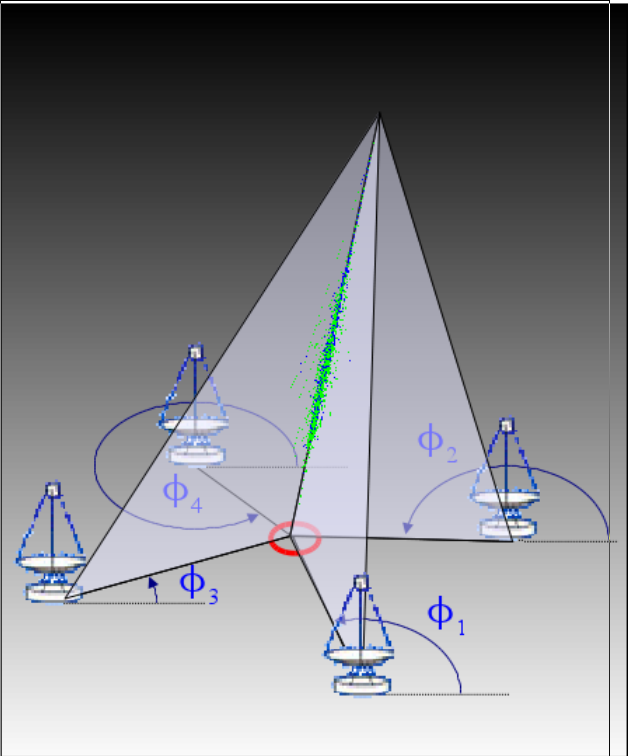
\includegraphics[width=0.6\textwidth]{images/hillas_reco.png}
	\caption{Illustration of a stereoscopic reconstruction of the source position.
    From each telescope a plane is drawn, the weighted intersection gives the interaction 
    point somewhere above the telescopes. The intersection of the projection to 
    the ground frame results in the core position (red circle). 
    The image is taken from a (Habitilations??) thesis by 
    Mathieu de Naurois \cite{hillas_reco}.}
	\label{fig:hillas_reconstructor}
\end{figure}

Since this method inherently requires a stereoscopic experiment
and multiple triggered telescopes, it will not work for a single telescope.
From earlier studies (see e.g. again \cite{kai_diss}), it is expected
that this method works best with an event multiplicity 
$\geq 3$ with higher multiplicity leading to better results.

In total, this step leads to the following features on array level:
\begin{itemize}
    \item{alt, az: Reconstructed source position}
    \item{core_x, core_y: Reconstructed source position}
    \item{alt, az: Reconstructed source position}
\end{itemize}

\section{High-Level Analysis}

\begin{center}
    \begin{tabular}{| l | l | l | l |}
    \hline
     & Pointlike Gamma & Diffuse Gamma & Protons \\
    \hline
    MC runs & \num{1113} & \num{17382} &  \num{9273} \\ 
    \hline
    Array events & \num{955317} & \num{3409290} & \num{4657529} \\
    \hline
    Telescope events & \num{4554313} & \num{14383270} \num{20106385} & 
    \end{tabular}
    \caption{Number of remaining events for each simulated particle type after the
    preprocessing. These are the numbers that get split into different datasets 
    and used for the machine learning tasks.}
    \label{tab:events_after_prep}
\end{center}


High level analysis of the preprocessed data is based on the use of
the aict-tools \cite{aict-tools} package which itself 
sklearn \cite{sklearn_api} for the implementation of the machine learning algorithms.
The aict-tools have originally been developed for the FACT-experiment
(citation needed) which is a single IACT. For this reason
adaptions had to be made compared to the status of the project at the start 
of this thesis to perform a stereoscopic analysis.
The algorithm of choice is the Random Forest algorithm
as it is well suited for the use with tabluar data and tends to rarely overfit
(citation needed).
Model feature importance will be calculated
based on the sklearn functionality, which
uses a XXX algorithm.
Separate models are trained for the tasks of gamma/hadron
separation and signal source position
reconstruction.


\subsection{Gamma-/Hadron-Separation}
For the task of gamma/hadron separation a random forest can be trained
using either only monoscopic information or also using array-level
information from earlier reconstruction steps.
Performance of the Classifier will be gauged based 
on the area under the receiver-operating-charateristic curve (AUC).
Using stereoscopic information
generally seems to improve the AUC by a few percent points.

The single telescope predictions can be combined by
simple functions such as the mean or median of the
single predictions to provide a prediction for the complete
array-event.

% features und kram


% \section{energy estimation}
% Energy estimation can be performed in the same way as the gamma/hadron
% separation. For this task there has been earlier work indicating
% the usefulness of a second machine learning model trained
% on the predictions of the first telesope-level model
% \cite{ba-lars}.

% I am thus going to present results based on either calculating the mean
% of the telescope level predictions and using a second random forest
% to improve the array level prediction.

\subsection{Reconstruction of the Source Position}
\label{sec:source_position}
The position on the shower axis can be estimated based on 
the hillas parameters and other image features, as 
explained in section \ref{??}
This method is known as the DISP-method in the
literature (citation needed). The general idea 
can be seen in figure \ref{fig:disp}.

\begin{figure}
    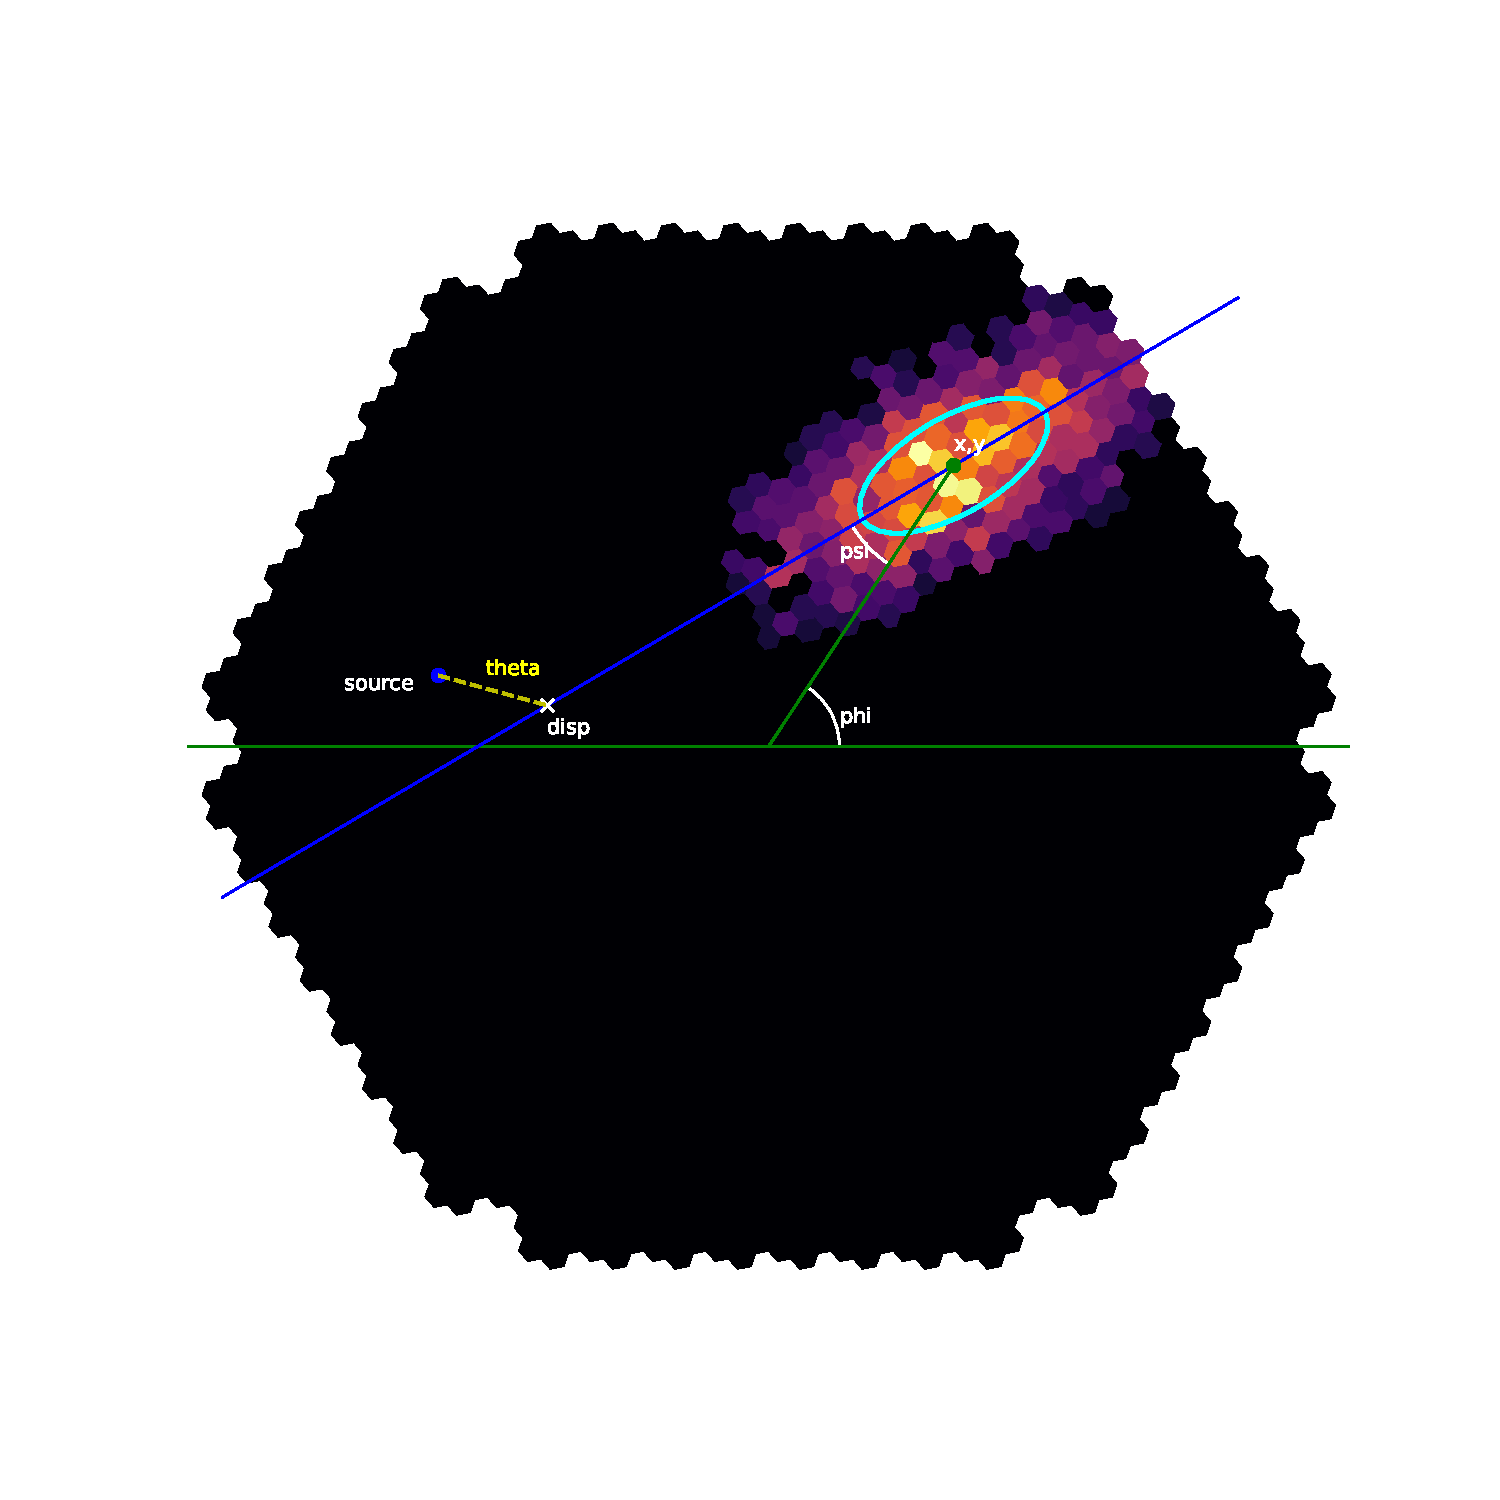
\includegraphics[width=0.6\linewidth]{Plots/hillas_complete.pdf}
    \caption{Illustration of monoscopic source position reconstruction making use of 
        the Hillas-Parameters and the DISP-method as explained in section \ref{sec:source_position}.
	A source position is estimated as some point on the main shower axis.
	In this example the head-/tail-ambiguation is guessed correctly.
	The position in the sky frame can then be calculated by transforming this
	point onto the sky plane.Pass das an zu 2 disps!}
    \label{fig:disp}
\end{figure}

With the DISP-method the estimated distance between the source
position and the center of gravity of the hillas ellipse gets calculated
based on the form of the ellipse, timing information and potentially
more features.
This will be done using machine learning models.
At this point the reconstructed source position
is fixed at two points at the main shower axis.

To resolve the head/tail ambiguity in monoskopic mode,
we will train a second random forest.
This is called SIGN-prediction, interpreting the two possible sides
as +-1, allowing for binary classification.
From FACT-analyses we know that accuracies of 70-80\% should be achievable
if we make no mistakes.

For the stereoskopic analysis, we employ an approach inspired by 
what the MAGIC-collaboration does in their analysis.
In the case of the MAGIC-telescopes the ambiguity does not
get resolved until the individual results get combined
on the stereo level. The choice of the correct
pair out of the four reconstructed positions can be done either
by calculating the crossing point of both main shower axises
or by calculating the pairwise distances between the positions \cite{magic disp paper}.


These methods are illustrated in figure \ref{fig:disp_magic}

\begin{figure}
    \begin{subfigure}{0.5\textwidth}
        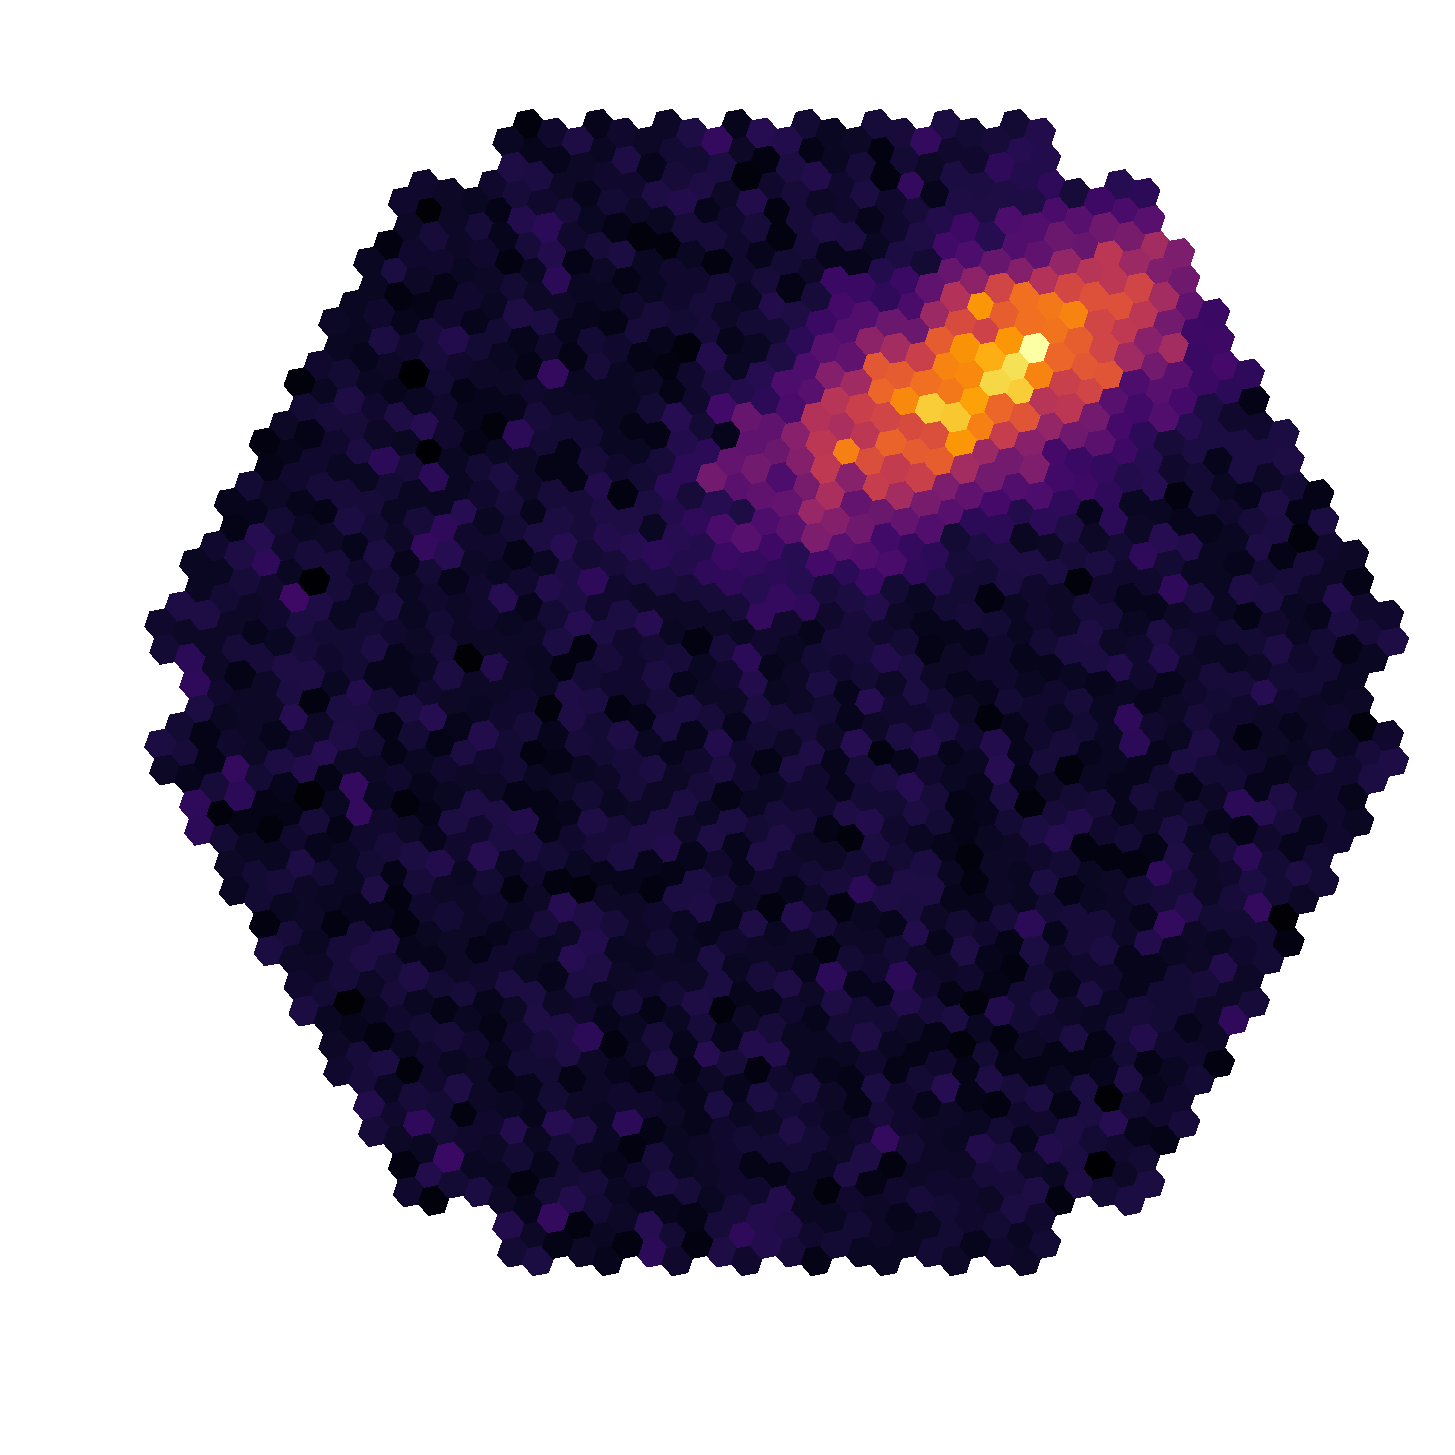
\includegraphics[width=0.9\linewidth]{Plots/hillas_raw.pdf} 
        %\caption{Caption1}
        \label{fig:3}
    \end{subfigure}
    \begin{subfigure}{0.5\textwidth}
        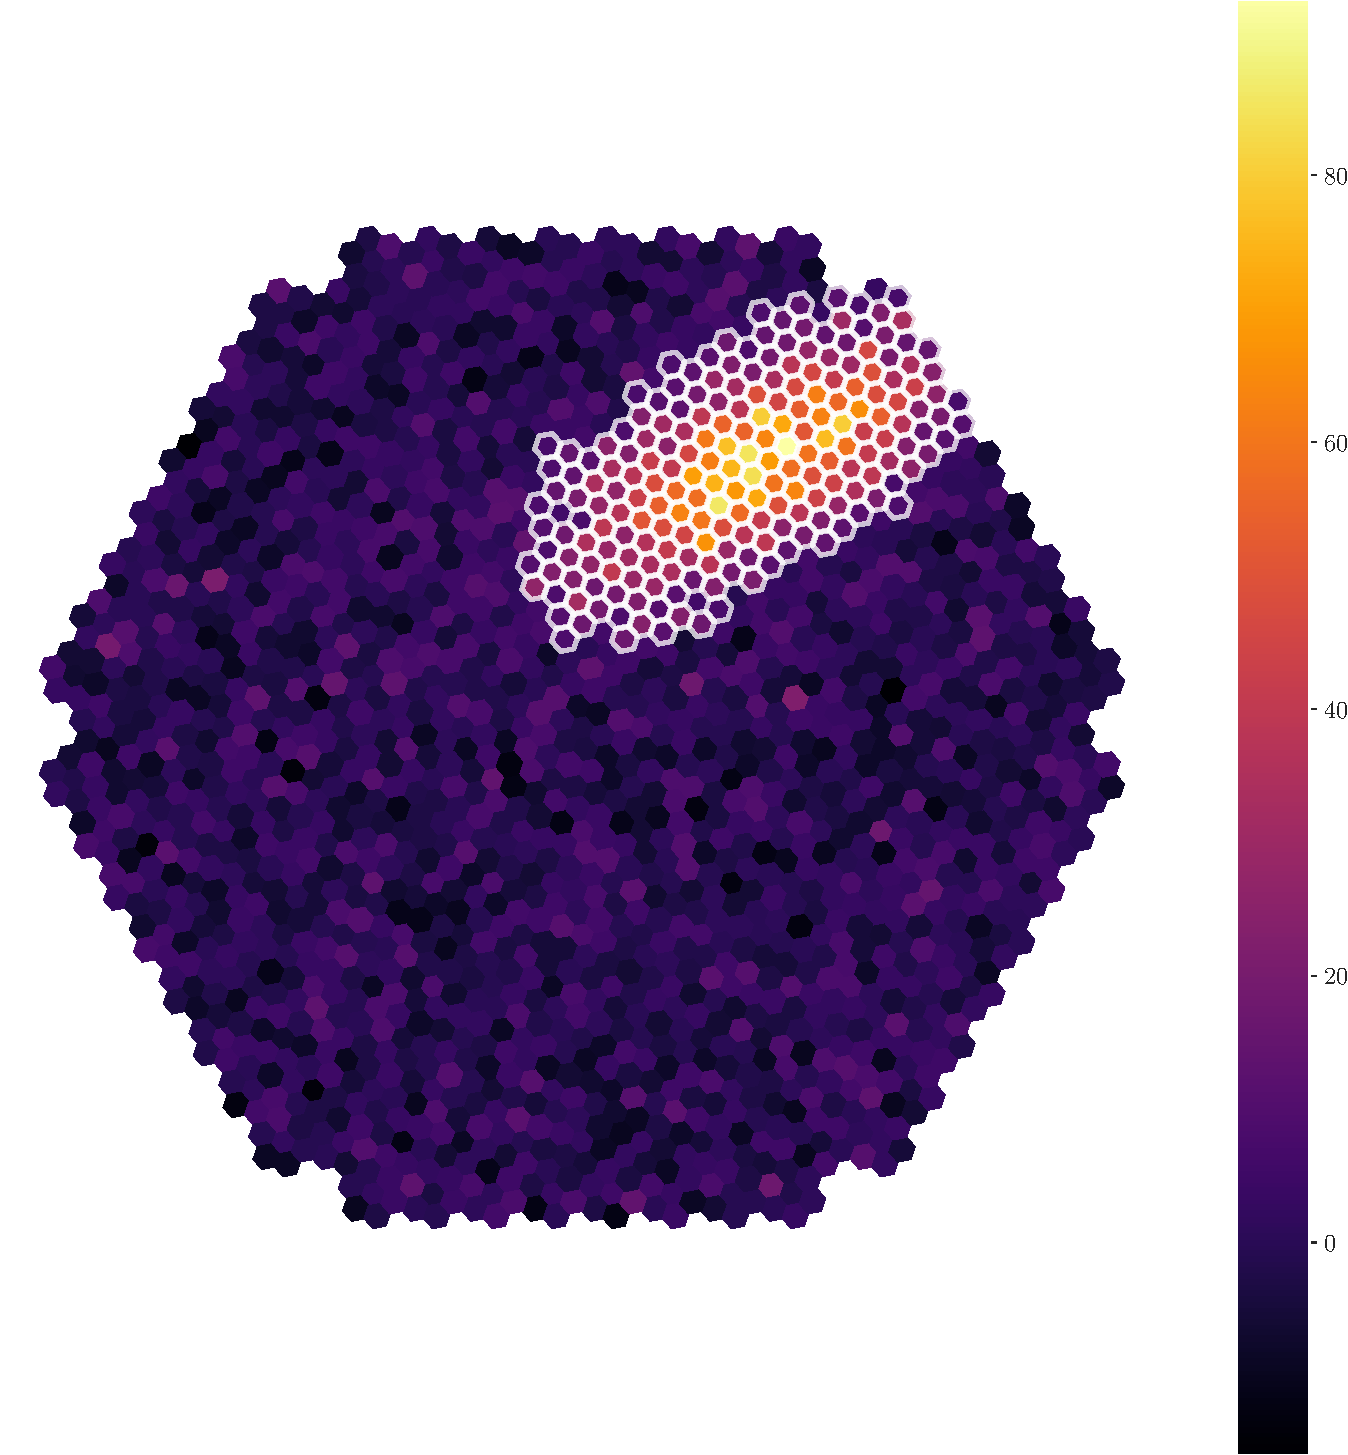
\includegraphics[width=0.9\linewidth]{Plots/hillas_cleaned.pdf}
        %\caption{Caption 2}
        \label{fig:2}
    \end{subfigure}
    \caption{wrong pics}
    \label{fig:disp_magic}
\end{figure}

Since we have a variable number of telescopes per (array) event,
we need to adapt this method in a scalable way.

The most obvious approach seemed to be an iterative one:
For each pair of triggered telescopes, we combine the results 
in the way described in \cite{disp magic paper}.
We cache all intermediate results and average them to get the final prediction.

Figure \ref{fig:stereo_disp} illustrates this for the case of 4 triggered telescopes.


\begin{figure}
    \begin{subfigure}{0.23\textwidth}
        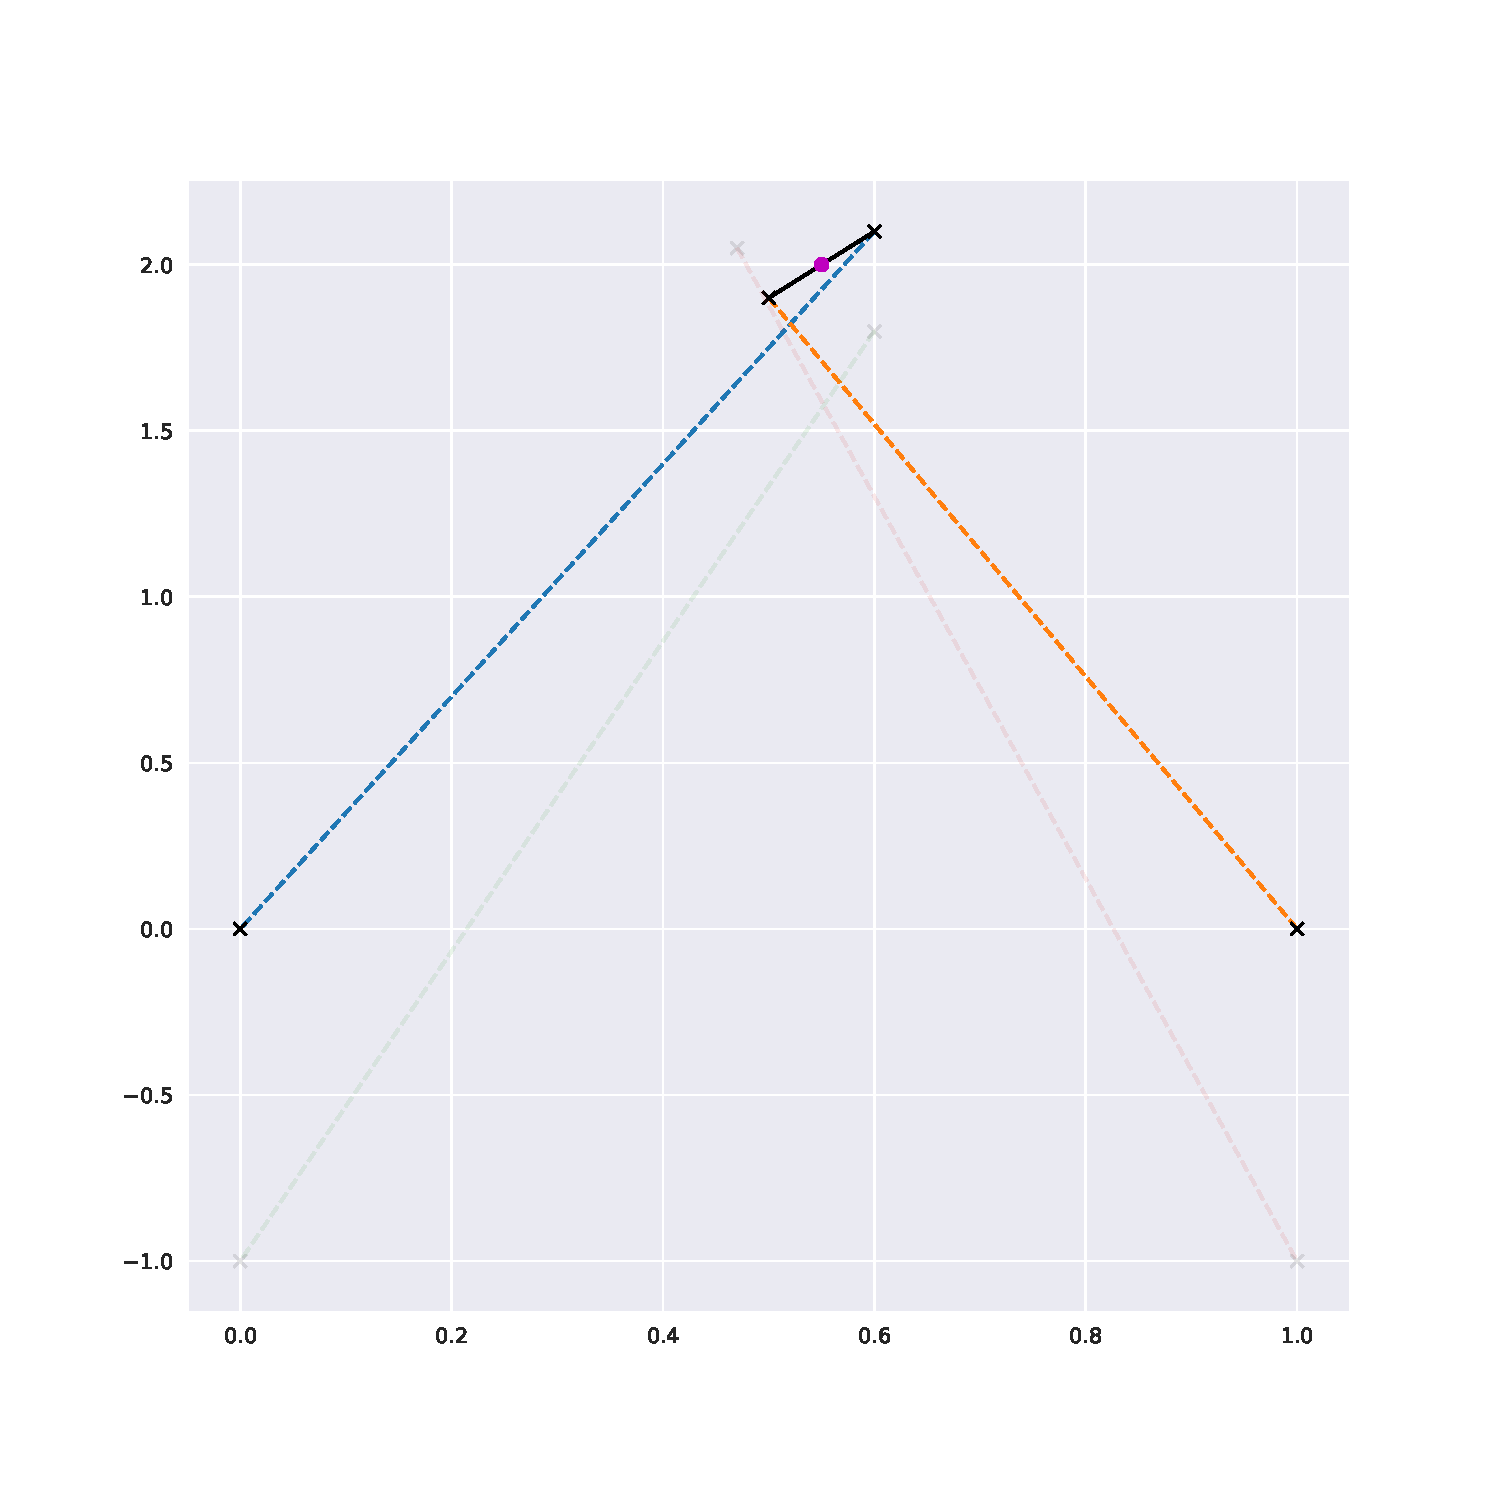
\includegraphics[width=0.9\linewidth]{Plots/stereo_magic_1.pdf} 
        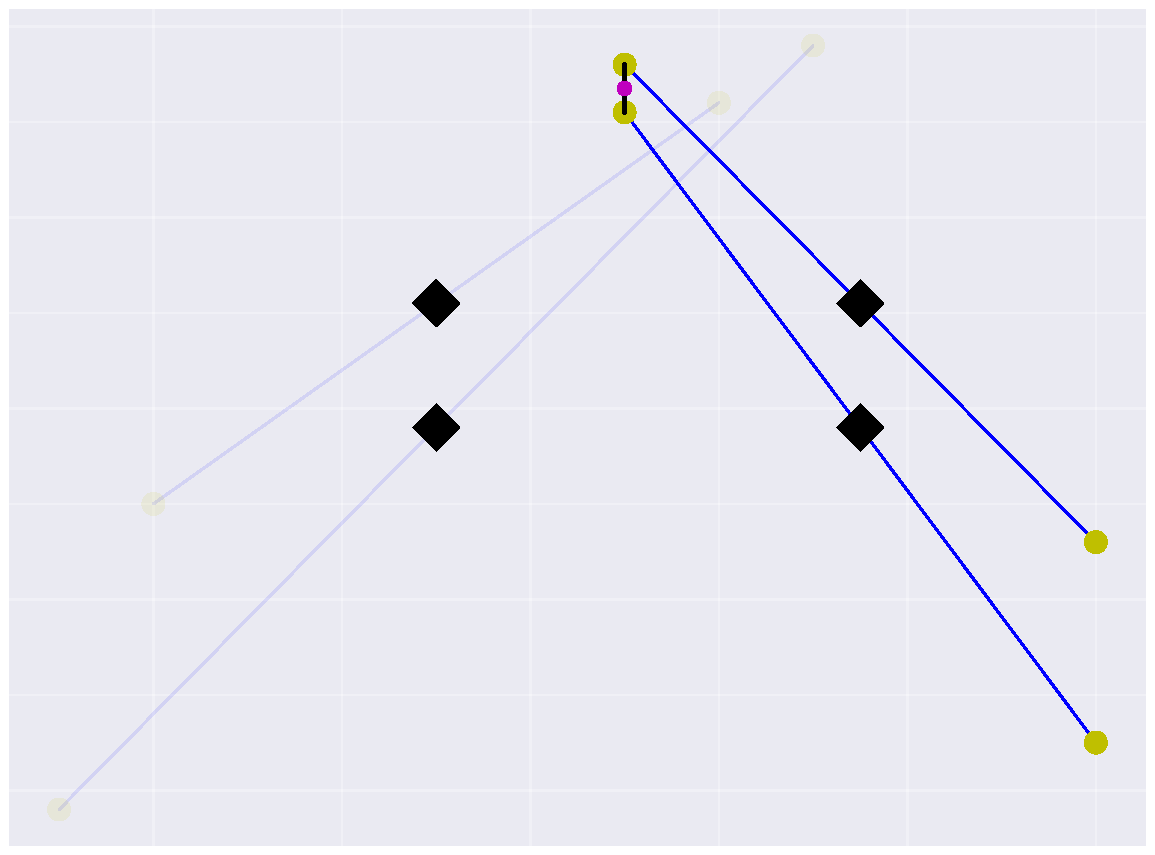
\includegraphics[width=0.9\linewidth]{Plots/stereo_magic_5.pdf} 
    \end{subfigure}
    \begin{subfigure}{0.23\textwidth}
        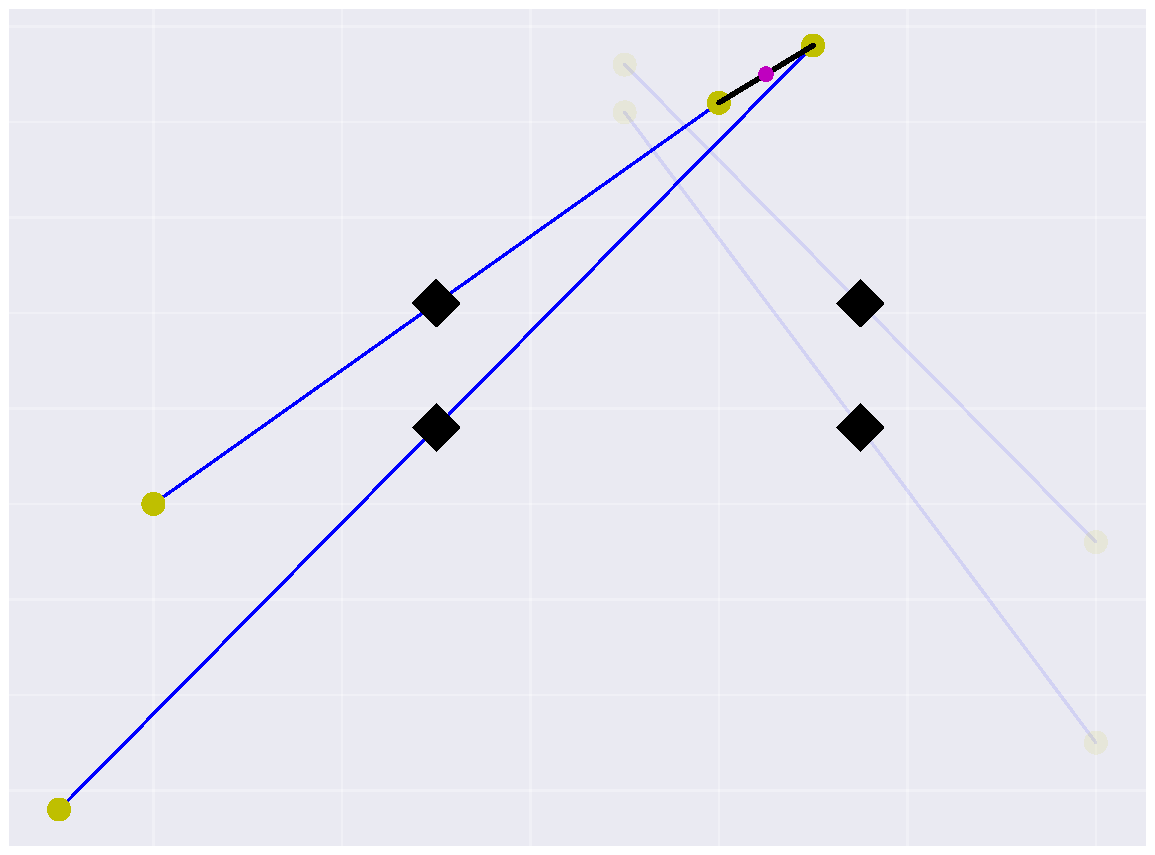
\includegraphics[width=0.9\linewidth]{Plots/stereo_magic_2.pdf}
        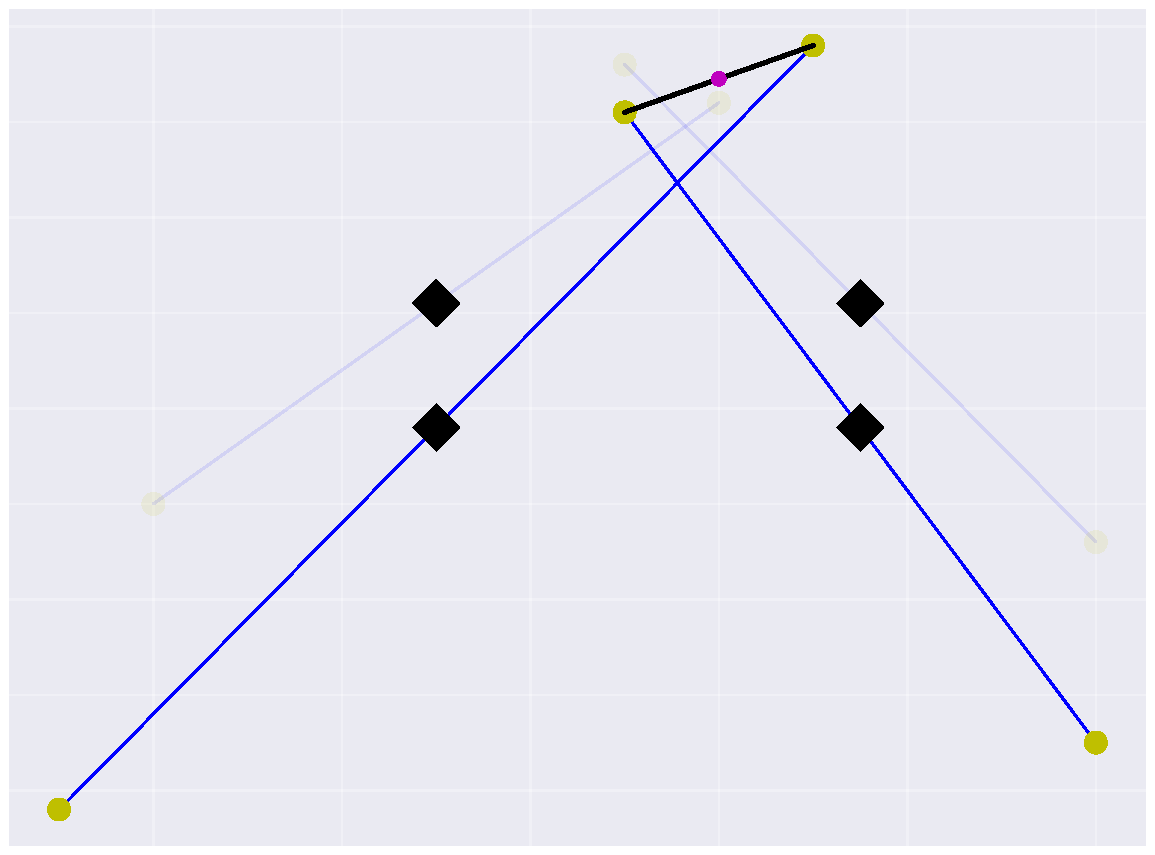
\includegraphics[width=0.9\linewidth]{Plots/stereo_magic_6.pdf}
    \end{subfigure}
    \begin{subfigure}{0.23\textwidth}
        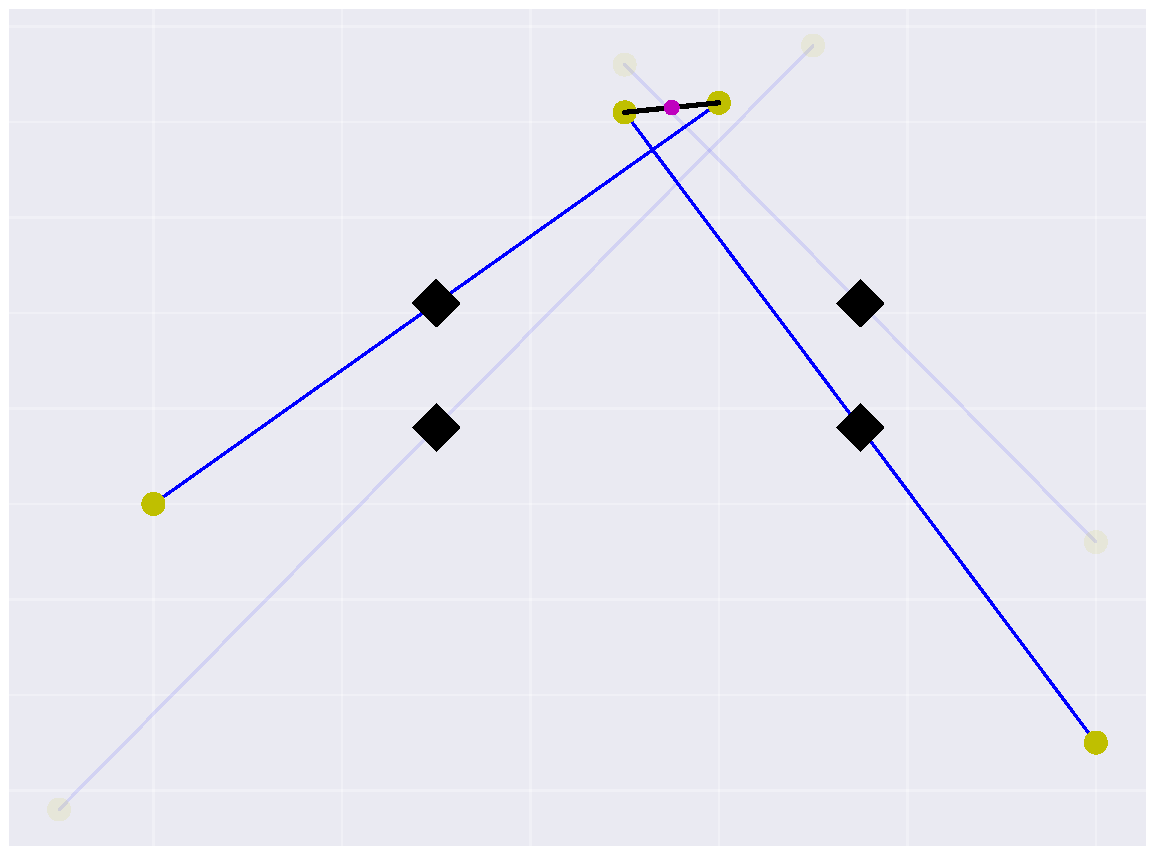
\includegraphics[width=0.9\linewidth]{Plots/stereo_magic_3.pdf} 
        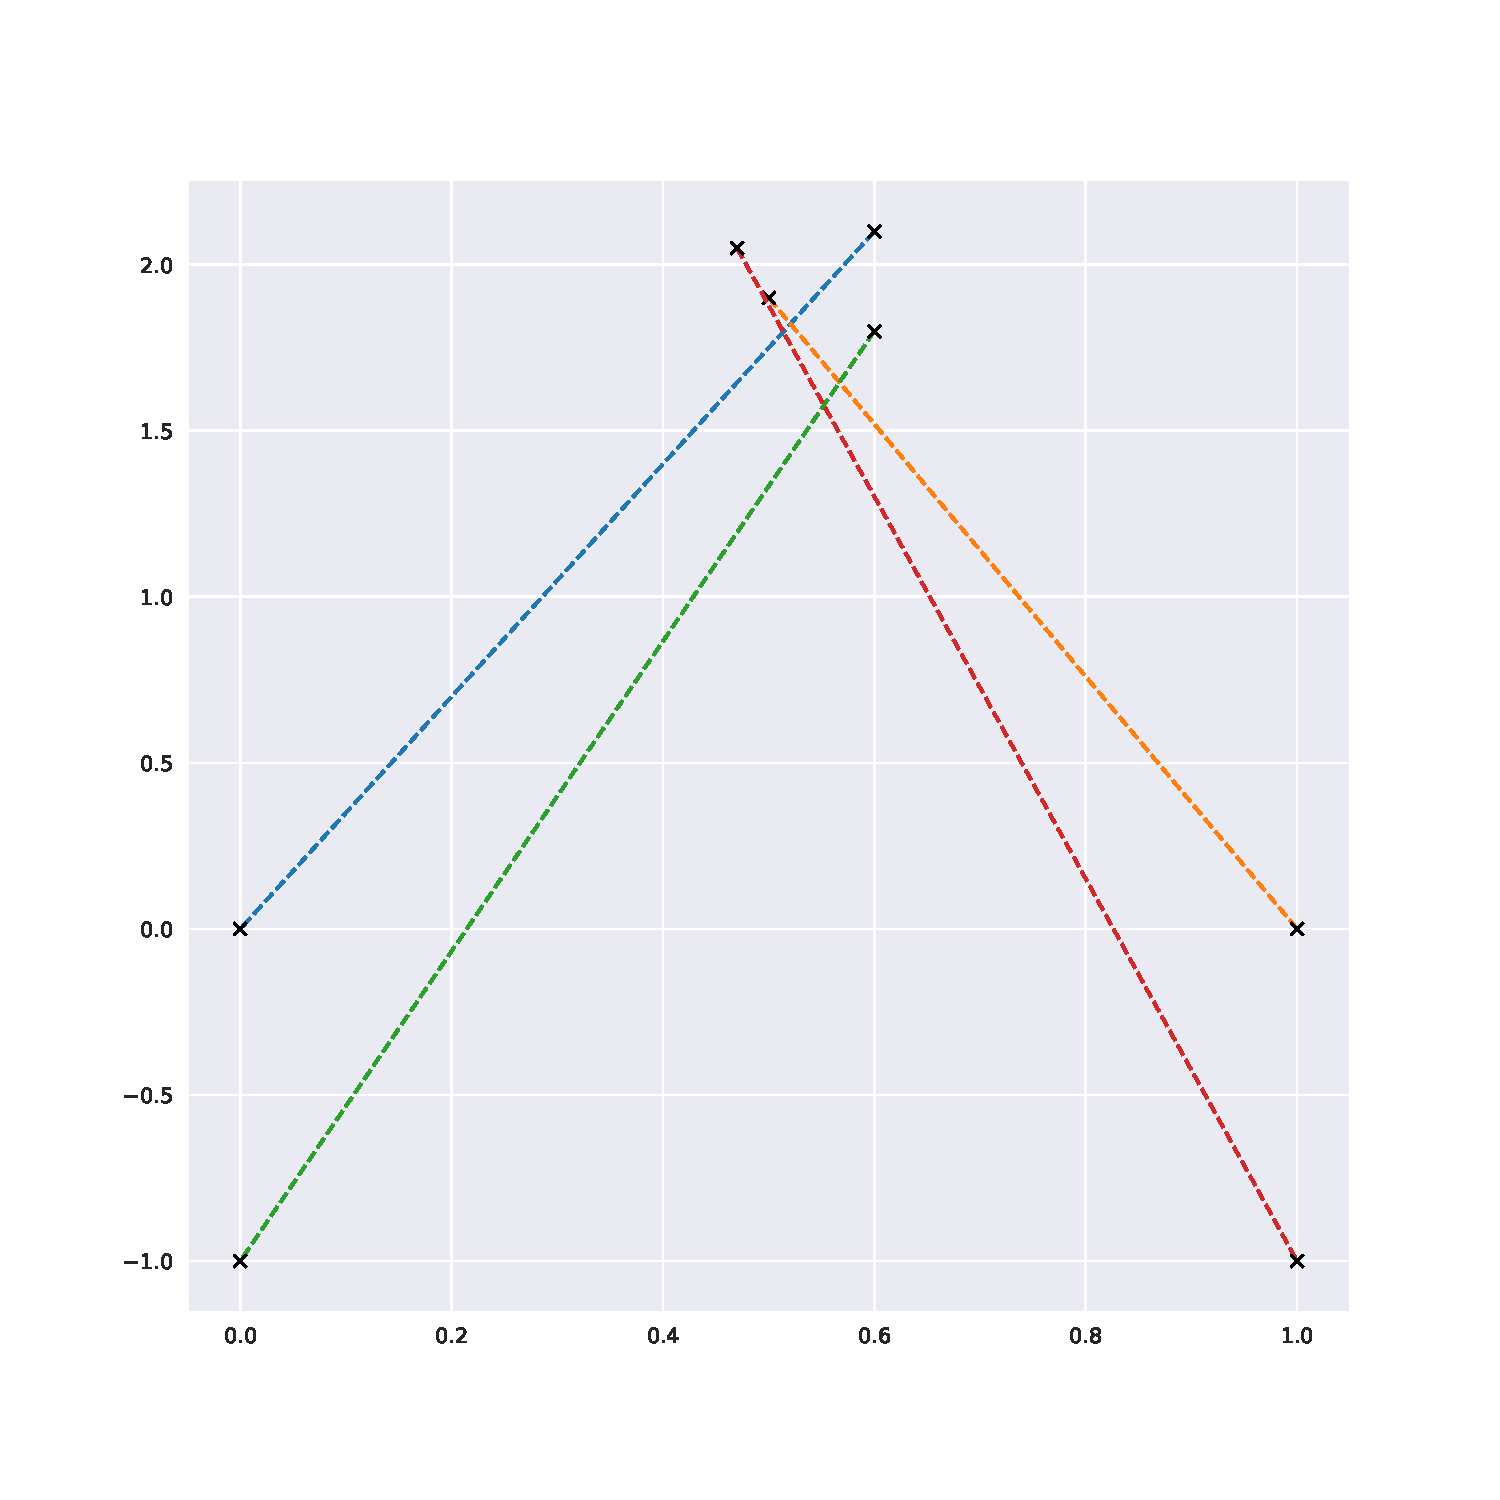
\includegraphics[width=0.9\linewidth]{Plots/stereo_magic_all.pdf} 
    \end{subfigure}
    \begin{subfigure}{0.23\textwidth}
        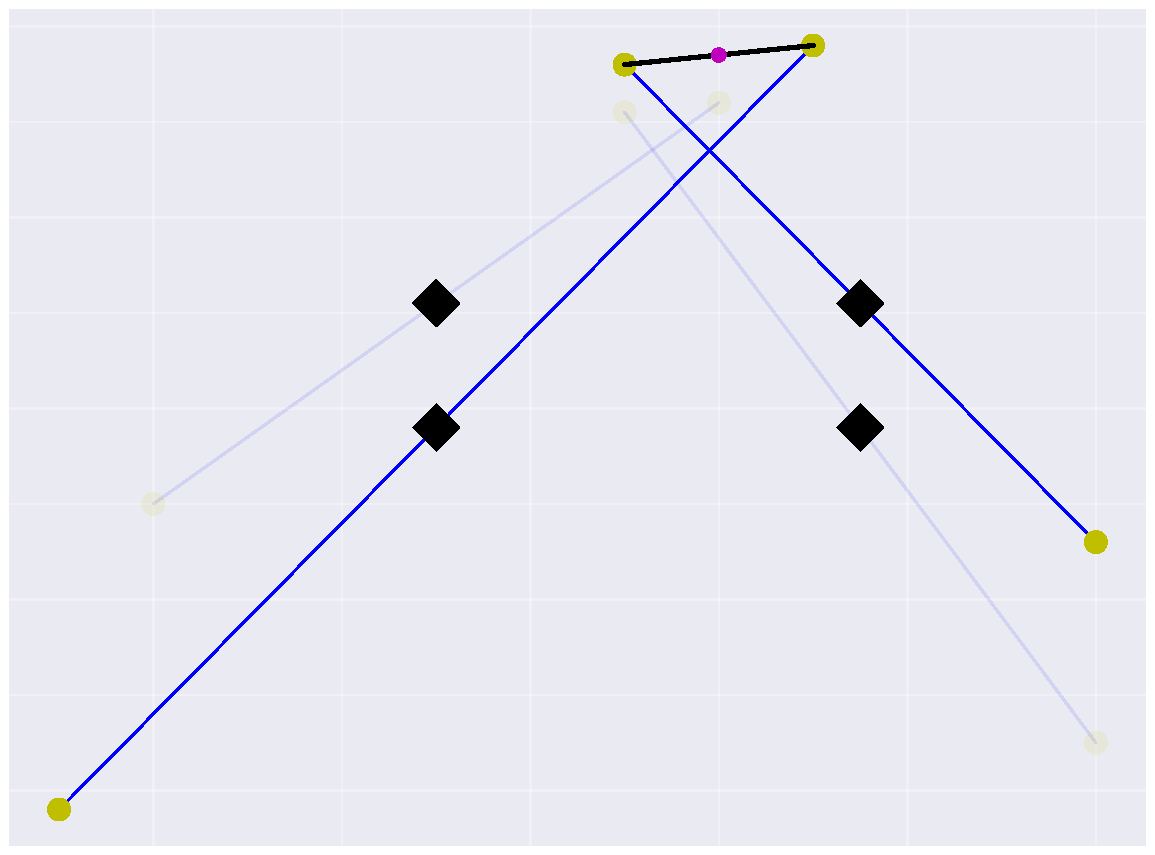
\includegraphics[width=0.9\linewidth]{Plots/stereo_magic_4.pdf}
        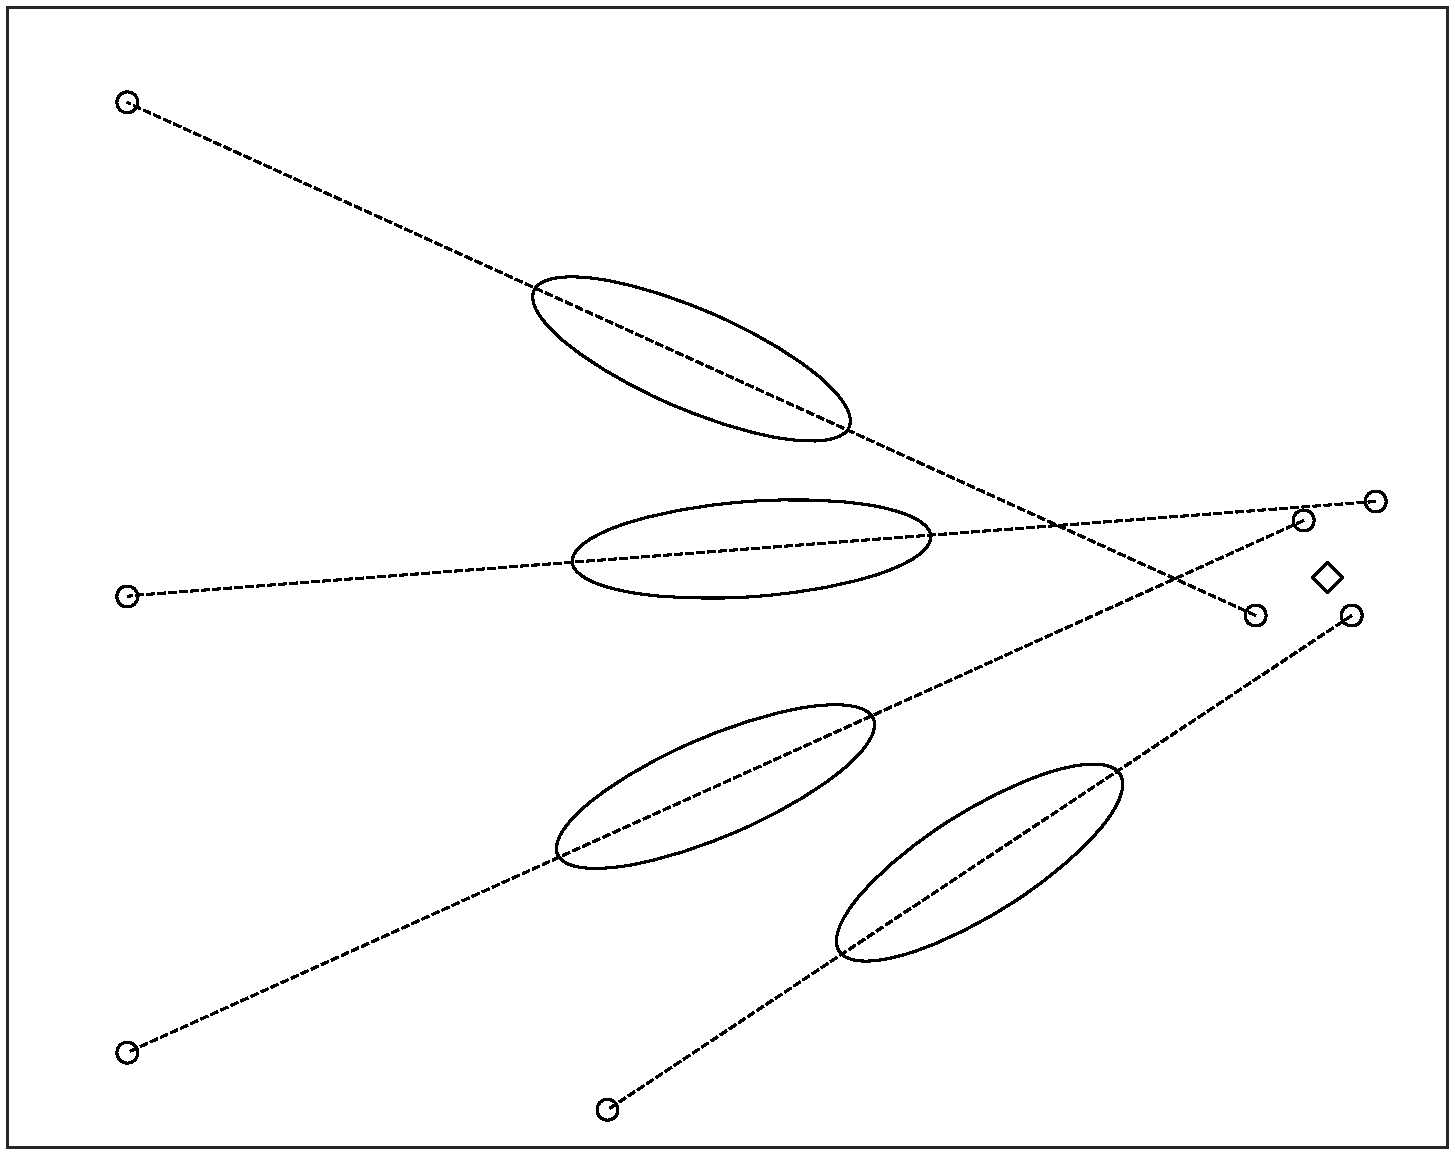
\includegraphics[width=0.9\linewidth]{Plots/stereo_magic_result.pdf}
    \end{subfigure}   \caption{wrong pics}
    \label{fig:stereo_disp}
\end{figure}


\section{Analysis for a single LST}